% =====================================================================
% GDRFA Dubai Scientific Research Award, second cycle (deadline 15 Oct 2026)
% Submission template following the official "Proposed Research Structure"
% and "Research Preparation & Formatting Requirements":
%   https://researchaward.gdrfad.gov.ae/guide-en.html  (read 10 Oct 2026)
%
% Rules from the guide (do not break):
%   * Length 4,000 to 8,000 words INCLUDING body, tables, figures,
%     appendices and references.            -> check with: bash wordcount.sh
%   * Upload MS Word file plus PDF.          -> bash build.sh ; bash to_docx.sh
%   * First page: title in both languages, researcher name(s), workplace,
%     job title, academic degree, email, contact number.
%   * Arabic abstract within 250 words; English abstract within 250 words.
%   * Language: English (Arabic allowed). Original, unpublished, not
%     submitted to another award this cycle.
%   * Structure (sections may be adjusted): 1 Title page, 2 Arabic abstract,
%     3 English abstract, 4 Introduction, 5 Research problem, significance
%     and objectives, 6 Theoretical and conceptual framework and literature
%     review, 7 Methodology and procedures, 8 Results, discussion and
%     analysis, 9 Conclusions and recommendations, 10 References,
%     11 Appendices (if any).
%
% Build: LuaLaTeX + BibTeX (babel handles Arabic). Self-contained for Overleaf: references.bib and figures/ live in this folder.
%
%
% Placeholders: \todo{...} prints grey italic guidance in the PDF.
% Set \showguidancefalse below to hide all guidance before submitting.
% =====================================================================
\documentclass[12pt,a4paper]{article}

% ---------- Engine check: the Arabic text needs LuaLaTeX ----------
\usepackage{iftex}
\ifluatex\else
  \errmessage{This document must be compiled with LuaLaTeX. In Overleaf: Menu > Compiler > LuaLaTeX, then Recompile}
  \stop
\fi

% ---------- Page and spacing ----------
\usepackage[margin=2.5cm]{geometry}
\usepackage{setspace}
\onehalfspacing
\setlength{\parskip}{0.4em}
\setlength{\parindent}{0pt}

% ---------- Content packages ----------
\usepackage{amsmath,amssymb}
\usepackage{graphicx}
\graphicspath{{figures/}}
\usepackage{booktabs}
\usepackage{array}
\usepackage{tabularx}
\usepackage{enumitem}
\setlist{itemsep=0.25em, topsep=0.3em}
\usepackage{caption}
\captionsetup{font=small, labelfont=bf}
\usepackage{float}
\usepackage{placeins}
\usepackage{pdflscape}
\usepackage[dvipsnames]{xcolor}
\usepackage{cite}
\usepackage{orcidlink}
\usepackage{fancyhdr}
\usepackage{titlesec}
\usepackage{xurl}
\usepackage{hyperref}
\hypersetup{hidelinks}
\newcolumntype{L}[1]{>{\raggedright\arraybackslash}p{#1}}

% ---------- Fonts and languages (LuaLaTeX + babel; Arabic direction stays local) ----------
\usepackage[english, bidi=basic]{babel}
\babelprovide[import]{arabic}
\babelfont{rm}{TeX Gyre Termes}
\babelfont[arabic]{rm}[Renderer=HarfBuzz, Scale=1.05]{Amiri}


% ---------- Headings: numbered as in the guide ----------
\titleformat{\section}{\large\bfseries}{\thesection.}{0.6em}{}
\titleformat{\subsection}{\normalsize\bfseries}{\thesubsection}{0.6em}{}
\titlespacing*{\section}{0pt}{1.2em}{0.5em}
\titlespacing*{\subsection}{0pt}{0.9em}{0.3em}

% ---------- Running header ----------
\pagestyle{fancy}
\fancyhf{}
\fancyhead[L]{\small GDRFA Dubai Scientific Research Award, second cycle}
\fancyhead[R]{\small Digital Innovation Award}
\fancyfoot[C]{\small\thepage}
\renewcommand{\headrulewidth}{0.4pt}
\setlength{\headheight}{14.5pt}

% ---------- Guidance placeholders ----------
\newif\ifshowguidance
\showguidancetrue   % set to \showguidancefalse before submission
\newcommand{\todo}[1]{\ifshowguidance\leavevmode{\color{gray}\itshape [#1]}\fi}

% ---------- Submission data (edit here once) ----------
\newcommand{\titleEN}{Refer or Clear: Reference-Conditioned Detection of Altered Travel Documents on Designs Never Seen}
\newcommand{\titleAR}{الإحالة أو التمرير: كشف التلاعب في وثائق السفر بالاستناد إلى مرجع التصميم، على تصاميم لم يسبق للنموذج رؤيتها}
\newcommand{\awardcategory}{Digital Innovation Award}
\newcommand{\awardtheme}{Artificial Intelligence: smart innovations and advanced data analytics}

\begin{document}

% =====================================================================
% 1. TITLE PAGE AND SUBMISSION DATA
% =====================================================================
\thispagestyle{empty}
\begin{center}
\singlespacing
{\normalsize\bfseries GDRFA Dubai Scientific Research Award, Second Cycle}\\[0.2em]
{\small \awardcategory}\\[1.2em]

{\large\bfseries \titleEN\par}
\vspace{0.8em}
\begin{otherlanguage}{arabic}
{\large\bfseries \titleAR\par}
\end{otherlanguage}
\vspace{0.4em}
\end{center}

{\small
\renewcommand{\arraystretch}{1.12}
\begin{tabularx}{\textwidth}{@{}L{2.7cm}>{\raggedright\arraybackslash}X>{\raggedright\arraybackslash}X@{}}
\toprule
 & \textbf{Researcher 1} & \textbf{Researcher 2} \\
\midrule
Name & Hamza A. Abushahla \orcidlink{0009-0003-6247-6776} & Ariel Justine N. Panopio \orcidlink{0009-0000-8168-6478} \\
Workplace & Computer Science and Engineering, American University of Sharjah & Computer Science and Engineering, American University of Sharjah \\
Job title & \todo{job title} & \todo{job title} \\
Academic degree & \todo{degree} & \todo{degree} \\
Email & b00090279@aus.edu & b00088568@aus.edu \\
Contact number & \todo{+971 ...} & \todo{+971 ...} \\
\midrule
 & \textbf{Researcher 3} & \textbf{Researcher 4} \\
\midrule
Name & \todo{name} & Mohamed I. AlHajri \orcidlink{0000-0003-1480-8054} \\
Workplace & \todo{workplace} & Computer Science and Engineering, American University of Sharjah \\
Job title & \todo{job title} & \todo{job title} \\
Academic degree & \todo{degree} & \todo{degree} \\
Email & \todo{email} & mialhajri@aus.edu \\
Contact number & \todo{+971 ...} & \todo{+971 ...} \\
\bottomrule
\end{tabularx}

\vspace{0.3em}
\begin{tabularx}{\textwidth}{@{}L{2.7cm}X@{}}
\toprule
Award category & \awardcategory \\
Theme & \awardtheme \\
Language & English \\
Word count & \todo{from wordcount.sh or Overleaf; 4,000 to 8,000 including tables, figures, appendices and references} \\
\bottomrule
\end{tabularx}
}

\vspace{0.5em}
{\footnotesize\textbf{Declaration.} This work is original, has not been published or accepted for publication in any journal or conference, and has not been submitted to another award in this cycle. The authors consent to its publication in the award's knowledge publications and electronic book.}

\onehalfspacing
\clearpage

% =====================================================================
% 2. ARABIC ABSTRACT (within 250 words)
% =====================================================================
\begin{otherlanguage}{arabic}
\section*{الملخص}
\end{otherlanguage}
\addcontentsline{toc}{section}{Arabic abstract}
\todo{Arabic abstract, at most 250 words. Translate the English abstract once it is final, and have a native speaker check the terminology: travel document, forgery, first line, Document Examination Centre.}
\medskip

\begin{otherlanguage}{arabic}
يعتمد ضابط الخط الأول على ثوانٍ معدودة ليقرر إحالة وثيقة السفر إلى مركز فحص الوثائق أو تمريرها.

\textbf{الكلمات المفتاحية:} وثائق السفر، كشف التزوير، التعلم العميق، الشبكات التوأمية، مراقبة الحدود.
\end{otherlanguage}
\vspace{1.5em}

% =====================================================================
% 3. ENGLISH ABSTRACT (within 250 words)
% =====================================================================
\section*{Abstract}
\addcontentsline{toc}{section}{English abstract}
\todo{At most 250 words. Structure: context (two-line document check at Dubai's border, centre figures); gap (no vendor publishes cross-design error rates; published detectors memorize designs); method (reference-conditioned detector built on a change-detection framework, design-median reference and zone mask); data and protocols (MIDV-2020, SIDTD, FantasyID; Protocol A and B, Arabic design); key results with numbers; implication for GDRFA. Source: abstract of ../main.tex, shortened.}

\textbf{Keywords:} travel documents; forgery detection; Siamese networks; change detection; border control; presentation attack detection.

\clearpage

% =====================================================================
% 4. INTRODUCTION
% =====================================================================
\section{Introduction}
\label{sec:intro}
\todo{About 600 words, deployment-motivated from the first sentence: the two-line check at Dubai's ports, seconds per document at a counter with a reader and a computer; the Document Examination Centre's own figures (902 irregularities in 20,307 examinations, a ratio among examined documents, not a prevalence); what the first line already operates (readers with a template library, a new design handled by adding its specimen); why the first-line decision is hard; one sentence on the approach; the structure of the paper. Source: ../main.tex Section 1 and the paper plan Section 2, items 1 and 2.}

% Example figure inclusion (figures are read from figures/):
% \begin{figure}[htbp]
%   \centering
%   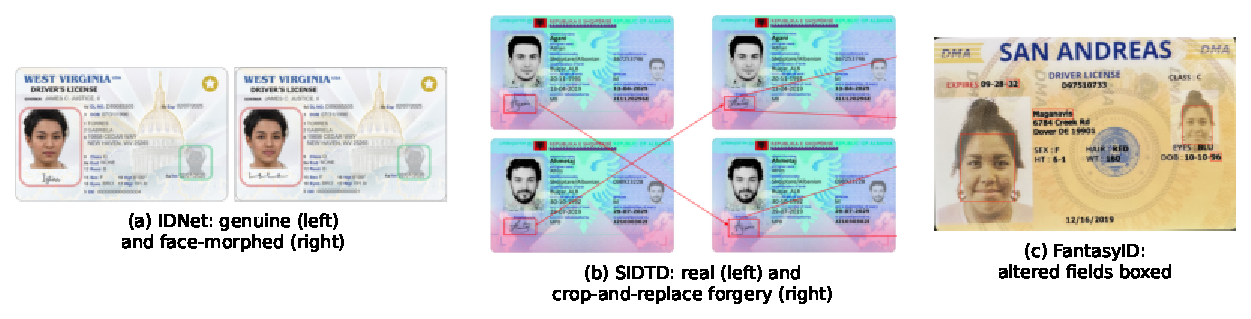
\includegraphics[width=\textwidth]{fig_attacks.pdf}
%   \caption{...}
%   \label{fig:attacks}
% \end{figure}

% =====================================================================
% 5. RESEARCH PROBLEM, SIGNIFICANCE AND OBJECTIVES
% =====================================================================
\section{Research Problem, Significance and Objectives}
\label{sec:problem}

\subsection{Research problem}
\todo{About 200 words. Refer or clear in seconds across 80+ countries' templates; we found no published cross-design error rate for the commercial readers; the detectors evaluated in the public benchmarks take one image and collapse on unseen designs. The gap sentence from the plan: the collapse is measured in four benchmarks; the specimen the counter already uses has never been given to a learned alteration detector and measured on those benchmarks against the same detector without it.}

\subsection{Significance}
\todo{About 200 words. For GDRFA: a measurement nobody publishes, a released protocol to repeat it on GDRFA's own template library, a new design handled by adding its specimen, a decision and a time budget on the counter computer. For the field: to our knowledge the first leave-design-out measurement of specimen conditioning for alteration detection on public data (reference-based detectors themselves are not new).}

\subsection{Objectives and research questions}
\todo{The aim and RQ1 to RQ5 (paper plan Section 2 and 5b).}
\begin{enumerate}[label=\textbf{RQ\arabic*.}]
  \item \todo{Loss of a single-image detector on unseen designs, and how much the reference recovers.}
  \item \todo{Gap between Protocol A and Protocol B, and what drives it.}
  \item \todo{Which fusion (stacked, difference, attention) and which reference construction (design median, single specimen, with and without the zone mask) carry the gain.}
  \item \todo{Referral rate at miss budgets of 1 and 5\%.}
  \item \todo{Whether the detector meets a first-line time budget on an ordinary CPU, and what the reference costs in time relative to the single-image model.}
\end{enumerate}

\subsection{Contributions}
\todo{Contributions C1 to C5 with their boundaries (paper plan Section 2b): the measurement, the method, the decision, the time budget, the release. Each states what it is not. Include the project-at-a-glance figure, fig\_pipeline.pdf, on a landscape page if space allows.}

% =====================================================================
% 6. THEORETICAL AND CONCEPTUAL FRAMEWORK AND LITERATURE REVIEW
% =====================================================================
\section{Theoretical and Conceptual Framework and Literature Review}
\label{sec:framework}

\subsection{Conceptual framework}
\todo{About 400 words. (i) First- and second-line inspection as defined by ICAO Doc 9303 and the Schengen Handbook; (ii) detection as a referral decision: referral rate $R(t)$ and miss rate $M(t)$ at a prior $p$, with the ISO/IEC 30107-3 error vocabulary; (iii) the reference-conditioning principle: comparing against a specimen turns single-image forensics into change detection, as in differential morph detection. Include the idea figure, fig\_idea.pdf, and the referral sketch, fig\_referral.pdf.}

\subsection{Literature review}
\todo{About 1,000 words in four strands, each closing with what it lacks; then the positioning paragraph and Table 1. Sources: ../main.tex Section 2 and the paper plan Sections 2, 2b and 5.}

\subsubsection{Single-image detectors and the measured collapse on unseen designs}
\todo{SIDTD few-shot (82 to 91 from 97 to 100 within design; CoAARC pairs a random genuine of any design and scores worst), IDNet cross-type (35 to 71), FantasyID held-out designs (faces AUC 56 to 62; 62\% of genuine referred to miss 5\% of attacks), DeepID (0.99 to 0.72 from fantasy to real IDs), DocForge-Bench (pixel F1 0.30), the 2026 survey (APCER above 24\% for every public model). Lacks: a way to use the specimen; a referral policy; a time budget.}

\subsubsection{Reference-conditioned detectors for documents}
\todo{CheckSim, Chen et al., Al-Ghadi and FMIDV (reference removed, AUC 0.5), Neitthoffer et al., Nieto-Hidalgo et al. 2026 prototypes; commercial template libraries. Lacks: leave-design-out evaluation on alterations with public data; a dense map; masks.}

\subsubsection{Deployment-oriented systems}
\todo{EdgeDoc, FLiD, the Idakto edge framework, vendor readers; DeepID container wall time. Lacks: any measured inference time or FPS; any cross-design error rate.}

\subsubsection{Where the architecture comes from: inspection and change detection}
\todo{Remote-sensing change detection (Daudt et al. 2018; Changer 2023, Open-CD); automated optical inspection against a golden sample (ChangeChip 2021; CADNet 2025; Visual ChangeNet); differential morphing-attack detection (Scherhag et al. 2020). Lacks: application to documents; a notion of legitimate variation (fields are supposed to differ), which the zone channel supplies.}

\subsubsection{Positioning and the gap}
\todo{The intersection in one paragraph, then Table 1 (positioning table from ../main.tex), then the gap sentence: the collapse is measured in four benchmarks; the specimen the counter already uses has never been given to a learned alteration detector and measured on those benchmarks against the same detector without it.}

% =====================================================================
% 7. METHODOLOGY AND PROCEDURES
% =====================================================================
\section{Methodology and Procedures}
\label{sec:method}
\todo{About 1,800 words. Keep the guide's wording: study population, samples, and tools.}

\subsection{Study population and samples}
\todo{The population is identity and travel documents presented at a first-line check; the samples are SIDTD (built on MIDV-2020; baseline-unmodified mock documents plus 1,222 generated forgeries), FantasyID (printed and captured fantasy cards, 13 designs, boxes with altered flags and a document quad per image) and IDNet's Arizona and West Virginia designs from the reduced Zenodo release (face morphing, portrait substitution, text attacks); sizes, designs, alteration classes, capture conditions and licences in a table; provenance-grouped splits (source plus donor); no real traveller's document. Source: docs/data-decision.md. Include fig\_templates.pdf.}

\subsection{Tools: data preparation}
\todo{Unified records; rectification by homography to the 512 x 800 canvas (FantasyID ships the quad); design-median reference with the query's identity excluded; zone mask from the original field rectangles; box masks from the altered rectangles; pairs, hard negatives with a wrong-design reference; the JPEG-quality audit across classes. No forgeries are generated by us.}

\subsection{Tools: proposed architecture}
\todo{Base framework ChangerEx (Open-CD), a transfer from change detection; where each block comes from (Daudt et al., Changer, Neitthoffer et al., TruFor and EdgeDoc; the class is golden-reference inspection); the zone-aware single-image baseline as the controlled comparison; standard variant (difference fusion) and improved variant (attention fusion); input, output, loss, training recipe. Include the architecture figure (TikZ in ../main.tex, Figure 6) as a PDF or redraw.}

\subsection{Evaluation protocols and metrics}
\todo{Protocols A, B and C (paper plan Section 3): A on SIDTD's official few-shot split (published rows measured on clips, ours on templates, stated); B zero-shot on FantasyID, headline on the three held-out designs with faces and text, Attack-1 separately with the Arabic cards broken out; C on IDNet's published West Virginia and Arizona pair, per task. Every table has three rows, text alterations, faces, all attacks; the claim rests on the first. The comparison table (Table 3 of ../main.tex, landscape); metrics: AUC, EER, APCER at BPCER 1 and 5\%, HTER at FantasyID's operating point, accuracy where published, pixel F1 and IoU on box masks, the transported referral threshold (primary) and referral at test miss 1 and 5\% (secondary).}

\subsection{Experiments}
\todo{Settings (single plus zones, stacked, difference, attention; ResNet-18; three seeds) and experiments E1 to E10 (experiments/README.md), with the priority order: A and B with the two core settings first, then the other two settings, then C.}

\subsection{Deployment measurement}
\todo{The model runs on the counter computer with the scanner as the sensor; the officer has seconds per document. Protocol: batch size one, FP32, CPU only, fixed thread count, 20 warm-ups then 200 timed documents; median and 95th percentile for pre-processing (decode, rectification, resize, zone lookup), network time with and without cached reference features, and end to end; parameters and file size; two named machines. Quantization and on-sensor execution are future work.}

% =====================================================================
% 8. RESULTS, DISCUSSION AND ANALYSIS
% =====================================================================
\section{Results, Discussion and Analysis}
\label{sec:results}
\todo{About 1,500 words. Every result as a table or figure; prose says what it means. Mean $\pm$ standard deviation over three seeds.}

\subsection{Protocol A: unseen design within a dataset}
\begin{table}[H]
\centering\small
\setlength{\tabcolsep}{4pt}
\caption{Protocol A (SIDTD nationality hold-out). Published rows from the SIDTD paper; our rows mean $\pm$ s.d. over three seeds.}
\label{tab:resA}
\begin{tabular}{llcccc}
\toprule
Method & Backbone & Acc. (\%) & AUC & EER (\%) & APCER@BPCER5 (\%) \\
\midrule
EfficientNet-B3 (published) & -- & 82.0 & 0.899 & -- & -- \\
ResNet50 (published) & -- & 90.6 & 0.963 & -- & -- \\
CoAARC (published) & -- & 62.8 & 0.675 & -- & -- \\
\midrule
Single image + zones (ours) & ResNet-18 & \todo{} & \todo{} & \todo{} & \todo{} \\
Channel-stacked (ours) & ResNet-18 & \todo{} & \todo{} & \todo{} & \todo{} \\
Difference fusion (ours) & ResNet-18 & \todo{} & \todo{} & \todo{} & \todo{} \\
Attention fusion (ours) & ResNet-18 & \todo{} & \todo{} & \todo{} & \todo{} \\
\bottomrule
\end{tabular}
\end{table}
\todo{Interpretation: how much of the single-image loss the reference recovers.}

\subsection{Protocol B: unseen dataset, generator, capture and script}
\begin{table}[H]
\centering\small
\setlength{\tabcolsep}{4pt}
\caption{Protocol B (FantasyID official test, zero-shot). Published rows from the FantasyID paper. $^\dagger$FantasyID counts bona fide as positive: its FNR is the share of genuine cards referred at an operating point missing about 5\% of attacks.}
\label{tab:resB}
\begin{tabular}{lccccc}
\toprule
Method & AUC all & AUC text & AUC face & HTER (\%) & Genuine referred (\%)$^\dagger$ \\
\midrule
TruFor (published) & 93.5 & 99.5 & 55.8 & 33.4 & 62.0 \\
MMFusion (published) & 94.4 & 99.8 & 61.5 & 25.8 & -- \\
TruFor (our re-run) & \todo{} & \todo{} & \todo{} & \todo{} & \todo{} \\
\midrule
Single image + zones (ours) & \todo{} & \todo{} & \todo{} & \todo{} & \todo{} \\
Difference fusion (ours) & \todo{} & \todo{} & \todo{} & \todo{} & \todo{} \\
Attention fusion (ours) & \todo{} & \todo{} & \todo{} & \todo{} & \todo{} \\
\bottomrule
\end{tabular}
\end{table}
\todo{Interpretation: the headline on the three held-out designs; Attack-1 on the seen designs with the Arabic cards broken out (no published counterpart at design level); faces in their own row with the reason the specimen is blind there and the live-face reference as the fix; the gap between protocols.}


\subsection{Protocol C: the published cross-type pair}
\begin{table}[H]
\centering\small
\setlength{\tabcolsep}{4pt}
\caption{Protocol C (IDNet, train on one design, test on the other; accuracy at threshold 0.5, per task). Published rows from the IDNet paper (arXiv 2408.01690 v2, Table 14), measured on the original images; ours on the reduced Zenodo release, one detector for all four tasks.}
\label{tab:resC}
\begin{tabular}{llcccc}
\toprule
Train $\rightarrow$ test & Method & Face morphing & Portrait subst. & Mixed & Text replacement \\
\midrule
WV $\rightarrow$ AZ & published (MixFaceNet-S / CNN) & 50.55 & 71.20 & 71.15 & 60.92 \\
WV $\rightarrow$ AZ & Single image + zones (ours) & \todo{} & \todo{} & \todo{} & \todo{} \\
WV $\rightarrow$ AZ & Difference fusion (ours) & \todo{} & \todo{} & \todo{} & \todo{} \\
\midrule
AZ $\rightarrow$ WV & published & 54.10 & 80.05 & 71.10 & 50.00 \\
AZ $\rightarrow$ WV & Single image + zones (ours) & \todo{} & \todo{} & \todo{} & \todo{} \\
AZ $\rightarrow$ WV & Difference fusion (ours) & \todo{} & \todo{} & \todo{} & \todo{} \\
\bottomrule
\end{tabular}
\end{table}
\todo{Interpretation: text replacement is the row the claim rests on; the face tasks are reported, not claimed.}

\subsection{Ablations and robustness}
\todo{Reference construction (median vs single specimen), zone mask on and off, fusion, attention bias; wrong-design reference with and without the gate; misregistration sweep 0 to 12 px; JPEG recompression at 90, 70, 50.}

\subsection{Referral analysis}
\todo{The transported policy: threshold calibrated on the source at a 5\% miss target, frozen, realized miss and referral on the unseen designs; the referral curves; prevalence scenarios at 0.1, 1 and 5\%; TruFor's published operating point (5\% missed, 62\% of genuine referred) as the comparator. No refer-everything baseline is claimed as current practice.}

\subsection{Inference time on CPU}
\begin{table}[H]
\centering\small
\setlength{\tabcolsep}{4pt}
\caption{Inference time per document on CPU (batch size one, FP32, median / p95 over 200 documents), throughput in documents per second (FPS, from the median end-to-end time), parameters and file size. Machines named in the text.}
\label{tab:timing}
\begin{tabular}{lccccccc}
\toprule
Variant & Params (M) & Size (MB) & Pre-proc. (ms) & Network (ms) & Network, cached ref. (ms) & End to end (ms) & FPS \\
\midrule
Single image + zones & \todo{} & \todo{} & \todo{} & \todo{} & -- & \todo{}& \todo{} \\
Difference fusion & \todo{} & \todo{} & \todo{} & \todo{} & \todo{} & \todo{}& \todo{} \\
Attention fusion & \todo{} & \todo{} & \todo{} & \todo{} & \todo{} & \todo{}& \todo{} \\
\bottomrule
\end{tabular}
\end{table}
\todo{Interpretation against the first-line budget; cost of the reference; what caching the reference features per design buys.}

\subsection{Discussion and limitations}
\todo{What the leave-design-out number measures and what it does not (two training generators; SIDTD negatives are mock documents; IDNet is the reduced release; capture tested only by FantasyID; masks are boxes); registration failures; faces; the Centre's ratio is not a prevalence; the four comparability caveats from the brief.}

% =====================================================================
% 9. CONCLUSIONS AND RECOMMENDATIONS
% =====================================================================
\section{Conclusions and Recommendations}
\label{sec:conclusions}
\todo{About 450 words. Conclusions tied to RQ1 to RQ5 and the results tables.}

\subsection*{Recommendations for GDRFA Dubai}
\todo{Each recommendation must follow from a result (evaluation criterion 7). Deployment: the measured CPU time supports running the detector on the existing counter computer beside the reader; quantization and execution on the scanner itself are future work. For example: request cross-design error rates from the reader vendor using the released protocol; calibrate the threshold on the centre's own template library; pilot the detector as a referral suggestion beside the existing checks; track referral and confirmed-hit rates per design as a KPI.}

% =====================================================================
% 10. REFERENCES (IEEE style; counted in the 8,000-word limit)
% =====================================================================
\FloatBarrier
\bibliographystyle{IEEEtran}
\bibliography{references}

% =====================================================================
% 11. APPENDICES (if any; counted in the 8,000-word limit)
% =====================================================================
\appendix
\section{Appendix: Dataset licences and access}
\todo{Optional. Licence and download route for each dataset, and the release terms of the derived data (CC BY-SA share-alike from MIDV-2020 and SIDTD).}

\end{document}
